\documentclass[11pt, oneside]{article}   	% use "amsart" instead of "article" for AMSLaTeX format
\usepackage{geometry}                		% See geometry.pdf to learn the layout options. There are lots.
\geometry{letterpaper}                   		% ... or a4paper or a5paper or ... 
%\geometry{landscape}                		% Activate for rotated page geometry
\usepackage[parfill]{parskip}    			% Activate to begin paragraphs with an empty line rather than an indent
\usepackage{graphicx}				% Use pdf, png, jpg, or eps§ with pdflatex; use eps in DVI mode
								% TeX will automatically convert eps --> pdf in pdflatex		
\usepackage{amssymb}
\usepackage{hyperref}
\usepackage{mathtools}
\usepackage{enumerate}
\usepackage{tikz}
\usepackage{pgf-pie} % Package to create pie charts
\usepackage{algorithm}   
\usepackage{algpseudocode} 
\usepackage{listings}
\usepackage{xcolor} % Optional: For custom colors
\usepackage{caption}
\newcommand{\ck}[1]{\textcolor{cyan}{CK: #1}}
\newcommand{\jc}[1]{\textcolor{orange}{JC: #1}}
\newcommand{\hm}[1]{\textcolor{blue}{HM: #1}}

\title{Homework 3 \\ CSC 277 / 477 \\ End-to-end Deep Learning \\ Fall 2024}
\author{Hanzhang Yin - \texttt{hyin12@u.rochester.edu}}
\date{}					


\begin{document}

\maketitle

\lstset{ 
    language=Python, % Specify language
    basicstyle=\ttfamily\footnotesize, % Font style
    keywordstyle=\color{blue}, % Keywords color
    commentstyle=\color{green!60!black}, % Comment color
    stringstyle=\color{red}, % String color
    numbers=left, % Line numbers on the left
    numberstyle=\tiny\color{gray}, % Line number style
    stepnumber=1, % Number every line
    numbersep=5pt, % Line number separation
    showstringspaces=false, % Don't show spaces in strings
    breaklines=true, % Break lines if necessary
    frame=single, % Frame around code
    captionpos=b, % Caption position (b for bottom)
    tabsize=4, % Tab size
}

\begin{center}
    \textbf{Deadline:} 10/31/2024
\end{center}


\section*{Instructions}

Your homework solution must be typed and prepared in \LaTeX. It must be output to PDF format. To use \LaTeX, we suggest using \url{http://overleaf.com}, which is free.

Your submission must cite any references used (including articles, books, code, websites, and personal communications).  All solutions must be written in your own words, and you must program the algorithms yourself. \textbf{If you do work with others, you must list the people you worked with.} Submit your solutions as a PDF to Blackboard. 


Your programs must be written in Python. The relevant code should be in the PDF you turn in. If a problem involves programming, then the code should be shown as part of the solution. One easy way to do this in \LaTeX \, is to use the verbatim environment, i.e., \textbackslash begin\{verbatim\} YOUR CODE \textbackslash end\{verbatim\}.








\clearpage

\section*{Problem 1: Distributed Model Training and Optimization Techniques (30 Points)}

\subsection*{Part(a): Benefits and Challenges of Distributed Model Training (10 points)} 
Distributed model training enables faster training times and allows scaling to larger datasets and models, but it also presents several challenges. Write a brief essay (around 200 words) addressing the following points:
\begin{itemize}
    \item \textbf{Benefits}: Discuss the advantages of distributed training, such as reduced training time, scalability, and the ability to handle large models and datasets that don’t fit on a single GPU. Include real-world examples (e.g., training models like GPT-3, BERT).
    \item \textbf{Challenges}: Explore the difficulties, including communication overhead, model synchronization, and potential bottlenecks like straggler nodes. Use real-world scenarios where distributed training is essential (e.g., cloud-based environments, large-scale NLP models).
\end{itemize}

\textbf{Answer:}
\\
\textit{Benefits: }
\\
Distributed model training allows for faster processing by parallelizing tasks across multiple machine, thus reducing the overall training time. 
This scalability enables the use of larger datasets and more complex models that would not fit on a single GPU, allowing researchers and engineers to tackle 
complicated modern deep learning challenges. For example, models like GPT-3 and BERT required vast resources, and distributed training across many GPUs is essnetial
to complete training in a reasonable timeframe. By distributed the workload, one can handle large-scale NLP models and other machine learning tasks more efficiently, 
leveraging cloud-based environments.
\\
\textit{Challenges: }
\\
Distributed training accelerates model training and handles large-scale datasets efficiently, but it introduces challenges like communication overhead between GPUs. Large models, such as BERT, require significant memory for parameters, optimizer states, and activations, necessitating distribution across GPUs. This distribution increases communication between devices, which can become a bottleneck, especially when models are large. Balancing communication costs with GPU compute power is crucial to ensure optimal performance, as one can become the limiting factor in different scenarios.
\\
Additionally, distributed training systems face issues like the "straggler problem," where slower nodes delay overall progress, and cloud-based environments are prone to hardware failures and network instability. Effective distribution of model and training data across GPUs is also essential. For instance, simple 2D parallelism can introduce data redundancy, limiting scalability. Designing efficient parallel strategies and carefully managing these bottlenecks is key to maximizing the performance of distributed training systems.

\newpage

\subsection*{Part(b): Mixed-Precision Training and Activation Checkpointing (10 points)} 
Distributed training often requires efficient memory and computational resource management. In this section, briefly discuss:
\begin{itemize}
    \item How \textbf{mixed-precision training} reduces memory usage and increases computational efficiency. Include a mathematical justification of how reducing the precision of floating-point operations can speed up training and lower memory requirements.
    \item How \textbf{activation checkpointing} trades off memory for additional computation. Use examples to illustrate how recomputing activations can reduce memory usage but increase computation time.
\end{itemize}

\textbf{Answer:}
\\
\textit{Mixed-Precision Training: }
\\
Mixed precision training combines FP32 and FP16 to optimize both memory usage and computational speed. In this approach, most operations, such as activations and gradient calculations, are performed in FP16, which significantly reduces memory consumption and accelerates matrix operations during forward and backward passes. However, model weights are typically kept in FP32 to prevent numerical instability and ensure training accuracy isn't compromised.
\\
Mathematically, reducing the precision of floating-point arithmetic decreases memory usage and data transfer bandwidth proportionally, allowing larger models to fit within GPU memory. This is crucial for training large-scale models, as it enables faster computation without a substantial loss in numerical accuracy. By leveraging the faster processing of FP16 operations while retaining the stability of FP32 weights, mixed precision training achieves a balance between speed and precision, resulting in efficient model training for deep learning tasks.

\textit{Activation Checkpointing: }
\\
Activation checkpointing trades off memory usage for increased computation time. Instead of storing all the intermediate activations during the forward pass (which consumes a lot of memory), only a subset of activations is saved.
During the backward pass, the stored activations are used, and the rest of the activations are recomputed when needed.
This approach reduces the memory footprint significantly at the cost of extra computation time, since recomputing activations adds overhead.
In a general scope, this technique is beneficial in training deep neural networks where memory is a limiting factor, allowing larger models to be trained with limited GPU resources.

\newpage

\subsection*{Part(c): Comparing DataParallel and DistributedDataParallel in PyTorch (10 Points)}
In this section, you'll explore two methods for multi-GPU training in PyTorch: \texttt{DataParallel} and \texttt{DistributedDataParallel}.
\begin{itemize}
    \item Read online tutorials on PyTorch's \href{https://pytorch.org/docs/stable/generated/torch.nn.DataParallel.html}{DataParallel} and \href{https://pytorch.org/tutorials/intermediate/ddp_tutorial.html}{DistributedDataParallel} methods. Starting with a single-GPU script, describe how to modify the code to enable DataParallel and to enable DistributedDataParallel. Focus on the changes needed in the \textbf{model definition} and \textbf{dataloader} (if required) and provide a \textbf{high-level description} of these changes.
    \item Compare \textbf{DataParallel} and \textbf{DistributedDataParallel} based on:  (1) The workload needed to modify the code; (2) Typical run time for training; (3) Which method is more flexible and can be used in more situations and why?
\end{itemize}
\\
\textbf{Answer:}
\\
\textit{(1):} 
\\
Enabling DataParallel: To modify a single-GPU PyTorch script to use DataParallel, minimal changes are required. For the model definition, you simply wrap the existing model with \texttt{torch.nn.DataParallel(model)}. This enables PyTorch to split the input data across multiple GPUs automatically and combine the results after processing. No major changes are required to the DataLoader, as the data splitting is handled by DataParallel.

\begin{verbatim}
# model
model = MyModel()

# Enable DataParallel
model = torch.nn.DataParallel(model)

# Rest of the code 
\end{verbatim}

Enabling DistributedDataParallel (DDP): Modifying a script to use DistributedDataParallel involves more effort. 
\\
First, the model needs to be wrapped with \texttt{torch.nn.parallel.DistributedDataParallel(model)}, but additional setup is needed, including initializing the process group using 
\\
\texttt{torch.distributed.init\_process\_group()} to coordinate communication between the GPUs. 
\\
Additionally, the DataLoader requires the use of \texttt{torch.utils.data.distributed.DistributedSampler} to ensure that each process receives a unique subset of the data for training.

\begin{verbatim}
import torch.distributed as dist

# init the process group
dist.init_process_group(backend='nccl')

# model
model = MyModel()

# Enable DistributedDataParallel
model = torch.nn.parallel.DistributedDataParallel(model)

# Use DistributedSampler in DataLoader
train_sampler = torch.utils.data.distributed.DistributedSampler(train_dataset)
train_loader = torch.utils.data.DataLoader(dataset=train_dataset, sampler=train_sampler)

# Rest of the code
\end{verbatim}

\textit{(2):} 
\\
DataParallel requires minimal changes to modify the code. Simply wrapping the model with \texttt{DataParallel} is sufficient, and there is no need to modify the \texttt{DataLoader}. In contrast, DistributedDataParallel requires more effort. It involves initializing process groups and using \texttt{DistributedSampler} in the \texttt{DataLoader}. The setup for DistributedDataParallel is more complex, especially in multi-node or cloud environments.
\\
In terms of training runtime, DataParallel tends to be slower. This is due to the overhead of replicating the model across all GPUs and the bottleneck created during gradient aggregation on the master GPU. The model is replicated across all GPUs at each step, which increases communication overhead. DistributedDataParallel, on the other hand, is faster and more efficient. It distributes the model only once and synchronizes gradients between GPUs, leading to better scalability across multiple GPUs, particularly in multi-node setups.
\\
When it comes to flexibility and use cases, DataParallel is easier to implement but less efficient. It is more suitable for smaller-scale training where simplicity of implementation is valued over speed. In contrast, DistributedDataParallel is more flexible and scalable, especially for large-scale training across multiple nodes. It is preferred for production-grade models and large distributed environments due to its superior efficiency and performance.

\newpage

\section*{Problem 2: Programming Task (30 Points)}
In this section, you will build upon the code from Homework 1, Problem 1.

\subsection*{Part(a) Effect of \texttt{num\_workers} in DataLoader: (10 Points)}
One important hyperparameter that affects training time in HW1 is \texttt{num\_workers}, found in train.py under \texttt{loader\_args}. In this task, you’ll explore how this parameter impacts data loading speed.

\textbf{Instructions:}
\begin{itemize}
    \item Measure the total run time for iterating through all batches in the \textbf{training set} as you increase \texttt{num\_workers} from 1 to 10.
    \item Since no model training is required, create a script with only the necessary components for data loading.
\end{itemize}

\textbf{Questions:}
\begin{itemize}
    \item What is the default value of \texttt{num\_workers} in \texttt{torch.utils.data.DataLoader}? What does this default setting mean?
    \item Plot the run time as \texttt{num\_workers} increases. What do you observe? Is the default setting optimal?
\end{itemize}
\\
\textbf{Answer:}
\begin{center}
    \includegraphics[width=0.7\textwidth]{graphs/Figure_1.png}
\end{center}
\\
\textit{Analysis: }
\\
The default value of num\_workers in torch.utils.data.DataLoader is 0, meaning that data loading happens synchronously in the main process without spawning additional worker processes. This setting minimizes multi-thread overhead but can result in slower loading, especially for large datasets or complex data transformations, as it doesn't leverage parallel processing.
\\
Based on the graph, we observe that the data loading time decreases significantly when the number of workers increases from 1 to 2, and then gradually increases as more workers are added. This suggests that for this specific dataset, having only 2 workers achieves the optimal balance between data loading efficiency and system overhead.
\\
This pattern is likely due to the relatively small dataset size. When using a small number of workers (like 2), the system can efficiently load the data without introducing significant overhead from managing multiple threads or processes. However, as the number of workers increases, the overhead of managing them (such as synchronization and communication) outweighs the benefits of parallelism, leading to longer loading times.

\textit{Code Implementation: }
\begin{lstlisting}
import time
import matplotlib.pyplot as plt
import torch
from torch.utils.data import DataLoader, Dataset
import pandas as pd
from torchvision import transforms
from PIL import Image
from tqdm import tqdm  # Progress tracking
    
class OxfordPetsDataset(Dataset):
    def __init__(self, dataframe, split, label_map, transform=None):
        self.dataframe = dataframe[dataframe['split'] == split]
        self.transform = transform
        self.label_map = label_map
    
    def __len__(self):
        return len(self.dataframe)
    
    def __getitem__(self, idx):
        # Debug: Check if image path is correct
        img_name = self.dataframe.iloc[idx]['image_name']
        img_path = f"Homework1/data/images/{img_name}"
        label = self.dataframe.iloc[idx]['label']
    
        try:
            image = Image.open(img_path).convert('RGB')  # Ensure image loads correctly
        except Exception as e:
            print(f"Error loading image: {img_path} - {e}")
            raise
    
        if self.transform:
            image = self.transform(image)
    
        return image, self.label_map[label]
    
def benchmark_num_workers(data_loader, num_batches):
    # In this case, I think using perf_counter rather than process_counter is preferred for benchmark testing.
    start_time = time.perf_counter()
    max_batches = min(num_batches, len(data_loader))
    
    for images, labels in tqdm(data_loader, total=max_batches, desc="Benchmarking"):
        pass  
    
    elapsed_time = time.perf_counter() - start_time
    print(f"Time for {max_batches} batches: {elapsed_time:.2f} seconds")
    return elapsed_time
    
def main():
    df = pd.read_csv('Homework1/problem_1/oxford_pet_split.csv')
    df['label_code'], unique_labels = pd.factorize(df['label'])
    label_map = dict(zip(unique_labels, range(len(unique_labels))))
    
    transform = transforms.Compose([
        transforms.Resize((224, 224)),
        transforms.ToTensor(),
    ])
    
    train_set = OxfordPetsDataset(dataframe=df, split='train', label_map=label_map, transform=transform)
    
    num_workers_list = range(1, 11)
    loading_times = []
    
    # Track outer loop progress
    for num_workers in tqdm(num_workers_list, desc="Testing num_workers"):
        loader = DataLoader(train_set, batch_size=8, num_workers=num_workers, shuffle=False)
    
        # Benchmark with 10 batches and log time
        time_taken = benchmark_num_workers(loader, num_batches=10)
        loading_times.append(time_taken)
    
    # Plot the results
    plt.plot(num_workers_list, loading_times, marker='o')
    plt.xlabel('Number of workers')
    plt.ylabel('Loading time (seconds)')
    plt.title('Effect of num_workers on DataLoader Performance')
    plt.grid(True)
    plt.show()
    
if __name__ == '__main__':
    main()  
\end{lstlisting}

\newpage

\subsection*{Part(b) Code Profiling: (10 Points)}
Profiling your code is crucial for optimizing deep learning models. In this task, you’ll analyze the runtime of different components during model development.

\textbf{Instructions:}
\begin{itemize}
    \item Modify train.py to record the \textbf{total time} spent in the following stages: (1) Data loading from the training DataLoader; (2) Model forward pass; (3) Loss calculation and backward pass; (4) Evaluation on the validation and test sets; (5)Other parts (i.e., overall runtime minus the above four parts).
    \item You can simply use \texttt{time.time()} or any profiling tool of your choice.
\end{itemize}

\textbf{Questions:}
\begin{itemize}
    \item Briefly explain your method for recording the time taken for loading training data.
    \item Create a pie chart showing the proportion of time spent on the five components. Also, present the results in a LaTeX table. Analyze the pattern, and propose one way to optimize training efficiency.
\end{itemize}

\textbf{Answer:}
\\
To measure the time spent on loading training data, time.time() function was used. The time was recorded at the point where inputs and labels are loaded into memory, and the difference between the start and end time was accumulated across all batches. Specifically, each batch in the training loop executed this logic:
\begin{lstlisting}
    start_time = time.time()
    inputs, labels = inputs.to(device), labels.to(device)
    data_loading_time += time.time() - start_time
\end{lstlisting}

\textit{Figure loaded in W \& B Terminal for runtime recoridng: }
The following running time is recorded with only \textbf{one} epoch of training using the code from Homework1 with slight modifications.
\\
\textbf{The graphs for the running result is being listed in the next page!}

\begin{center}
    \includegraphics[width=0.9\textwidth]{graphs/Figure_2.png}
\end{center}

\begin{figure}[ht]
    \centering
    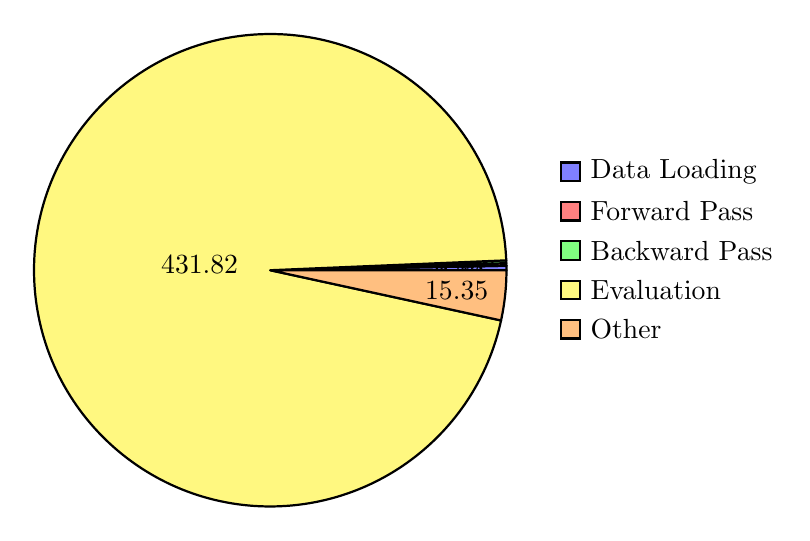
\begin{tikzpicture}
        \pie[
            text=legend, % Display legend with labels
            radius=3, % Size of the pie chart
            color={blue!50, red!50, green!50, yellow!50, orange!50},
            sum=auto % Automatically sum percentages
        ]{
            1.37/ Data Loading,
            0.78/ Forward Pass,
            0.85/ Backward Pass,
            431.82/ Evaluation,
            15.35/ Other
        }
    \end{tikzpicture}
    \caption{PieChart: Proportion of Time Spent on Training Components / Unit: seconds}
    \label{fig:time_pie_chart}
\end{figure}

\begin{table}[ht]
    \centering
    \begin{tabular}{|l|c|}
    \hline
    \textbf{Component}      & \textbf{Time (seconds)} \\ \hline
    Data Loading            & 1.37                    \\ \hline
    Forward Pass            & 0.78                    \\ \hline
    Backward Pass           & 0.85                    \\ \hline
    Evaluation              & 431.82                  \\ \hline
    Other                   & 15.35                   \\ \hline
    \textbf{Total Runtime}  & 450.18                  \\ \hline
    \end{tabular}
    \caption{Table: Time Spent on Each Component During Training / Unit: seconds}
    \label{tab:time_components}
\end{table}

\textit{Analysis: }
\\
The results indicate that \textbf{evaluation time} dominates the total runtime, accounting for \textbf{over 95\%} of the time, while \textbf{data loading, forward pass, and backward pass} take up minimal portions. To \textbf{optimize training efficiency}, the evaluation frequency can be reduced by conducting it every few epochs or steps instead of after every epoch. Additionally, using \textbf{smaller validation datasets} for intermediate evaluations or employing \textbf{asynchronous evaluation} methods can further minimize evaluation overhead. These adjustments would allow more time for model training, accelerating the process while maintaining effective performance monitoring.

\newpage

\subsection*{Part(c) Automatic Mixed Precision Training: (10 Points)}
In this task, you'll explore mixed precision training using \texttt{torch.amp}. Follow \href{https://pytorch.org/docs/stable/notes/amp_examples.html}{this tutorial}, focusing on the ``Typical Mixed Precision Training" section. Modify your code to enable mixed precision training.

\textbf{Instructions:}
\begin{itemize}
    \item Compare the following aspects using your WandB logs: (1) Training loss dynamics; (2) Final model performance; (3) System metrics, including GPU memory usage, total run time, and other relevant logs you found interesting under the ``System" section in Wandb (these are automatically logged by Wandb during the experiments; x-axis in these plots indicates runtime).
\end{itemize}

\textbf{Questions:}
\begin{itemize}
    \item What did you observe in terms of training loss, final performance, and system metrics? What conclusions can you draw from these experiments?
\end{itemize}

\textbf{Answer:}
\\
\begin{figure}[h!]
    \centering
    \includegraphics[width=0.9\textwidth]{graphs/Figure_3.png}
    \caption{AMP Model Performance Metrics}
    \label{fig:amp_metrics}
\end{figure}

\begin{figure}[h!]
    \centering
    \includegraphics[width=0.9\textwidth]{graphs/Figure_4.png}
    \caption{AMP Model System Charts}
    \label{fig:amp_system}
\end{figure}

\textit{Analysis: }
The comparison between the \textbf{AMP-enabled model} and the \textbf{non-AMP model} reveals several key insights regarding \textit{training loss dynamics}, \textit{final performance}, and \textit{system metrics}. Both models exhibit a steady decline in \textbf{training loss}, indicating effective learning. However, fluctuations in the later stages suggest potential room for fine-tuning the model's hyperparameters or increasing the training epochs to improve convergence. The \textbf{final test accuracy} for both models remains around \textbf{40\%}, indicating that additional adjustments, such as increasing the number of epochs or refining the learning rate, could lead to better performance.
\\
In terms of system resource usage, the \textbf{AMP model} shows clear advantages. By utilizing \textbf{mixed precision}, the model efficiently manages GPU memory, maintaining stable GPU usage and reducing memory overhead. This results in \textbf{faster computation} while preserving similar model performance. Despite these benefits, the observed variability in \textbf{CPU usage} suggests potential bottlenecks during data loading, which could slow down the overall training process. Additionally, the steady increase in \textbf{network traffic} across both models indicates potential overhead from logging operations or dataset access.
\\
To further optimize training, improvements could focus on \textbf{asynchronous data loading} to reduce CPU-bound operations, \textbf{increasing the number of training epochs} for better convergence, and fine-tuning the \textbf{batch size and learning rate} to balance resource utilization and performance. Furthermore, reducing frequent network logging can streamline the training process, improving both speed and accuracy. Ultimately, while \textbf{AMP} offers significant benefits in memory efficiency, these additional optimizations are essential to fully leverage the model's potential and system resources.

\end{document}   